\documentclass[11pt,a4paper]{article}
\usepackage[margin=18mm]{geometry}
\usepackage[T1]{fontenc}
\usepackage{lmodern}
\usepackage{amsmath,amssymb,graphicx,booktabs}
\usepackage[hidelinks]{hyperref}
\usepackage{microtype}
\setlength{\parindent}{0pt}
\setlength{\parskip}{4pt}
% Generated from full-precision saved evidence.
\newcommand{\KawaRateLower}{0.999850032944}
\newcommand{\KawaRateUpper}{0.999850618714}
\newcommand{\KawaOpenRadius}{0.999850032944}
\newcommand{\KawaTimingStates}{48}
\newcommand{\KawaTimingCalls}{960}
\newcommand{\KawaTimingWarmups}{96}
\newcommand{\KawaMatlabRelease}{2025b}


\newcommand{\comment}[1]{\smallskip\textbullet\ #1\par}
\newcommand{\panelnote}[1]{{\small #1\par}}
\newcommand{\fullfigure}[1]{\begin{center}
\includegraphics[width=\linewidth,height=.84\textheight,keepaspectratio]{figures/#1.pdf}
\end{center}}
\newcommand{\trajectorycase}[1]{
\clearpage
\section*{3D trajectories, #1x initial error}
\panelnote{First twelve cycles on each controller's exact switching grid.
The black circle is the shared initial state; the star is the cycle anchor.}
\fullfigure{state_space_#1x}
\clearpage
\section*{Trajectory projections, #1x initial error}
\panelnote{The same continuous-time paths in three coordinate planes.
Open circles mark actual cycle-start states, $k=0,\ldots,12$.}
\fullfigure{trajectory_projections_#1x}
\clearpage
\section*{Voltages and current, #1x initial error}
\panelnote{First twelve cycles. Each response keeps its own switching grid;
the reference retains its periodic ripple.}
\fullfigure{physical_states_#1x}
\ifnum#1>1\relax
\comment{This case starts with negative current. It is a mathematical stress
test, not a validated operating condition.}
\fi
\ifnum#1=3\relax
\comment{MPC-5 also crosses below $v_{C_1}=0$. Dwell feasibility does not enforce state limits.}
\fi
}

\begin{document}
\begin{center}
{\Large Three switching-time controllers, one converter\par}
Current LQR, MPC-5, and Common-P gain synthesis
\end{center}

\section*{Convergence speed}
\panelnote{Same converter and weights, 100 exact cycles, $T=286\,\mu\mathrm{s}$.
The 1x case is the article's initial error; 2x and 3x scale its displacement
from the cycle anchor. Shorter bars mean faster convergence. Outlined bars are fastest.}
\panelnote{The measured threshold is $E_k<0.01$, maintained through the rest
of the saved 100-cycle run. Times use actual cycle-start samples.}
\begin{center}
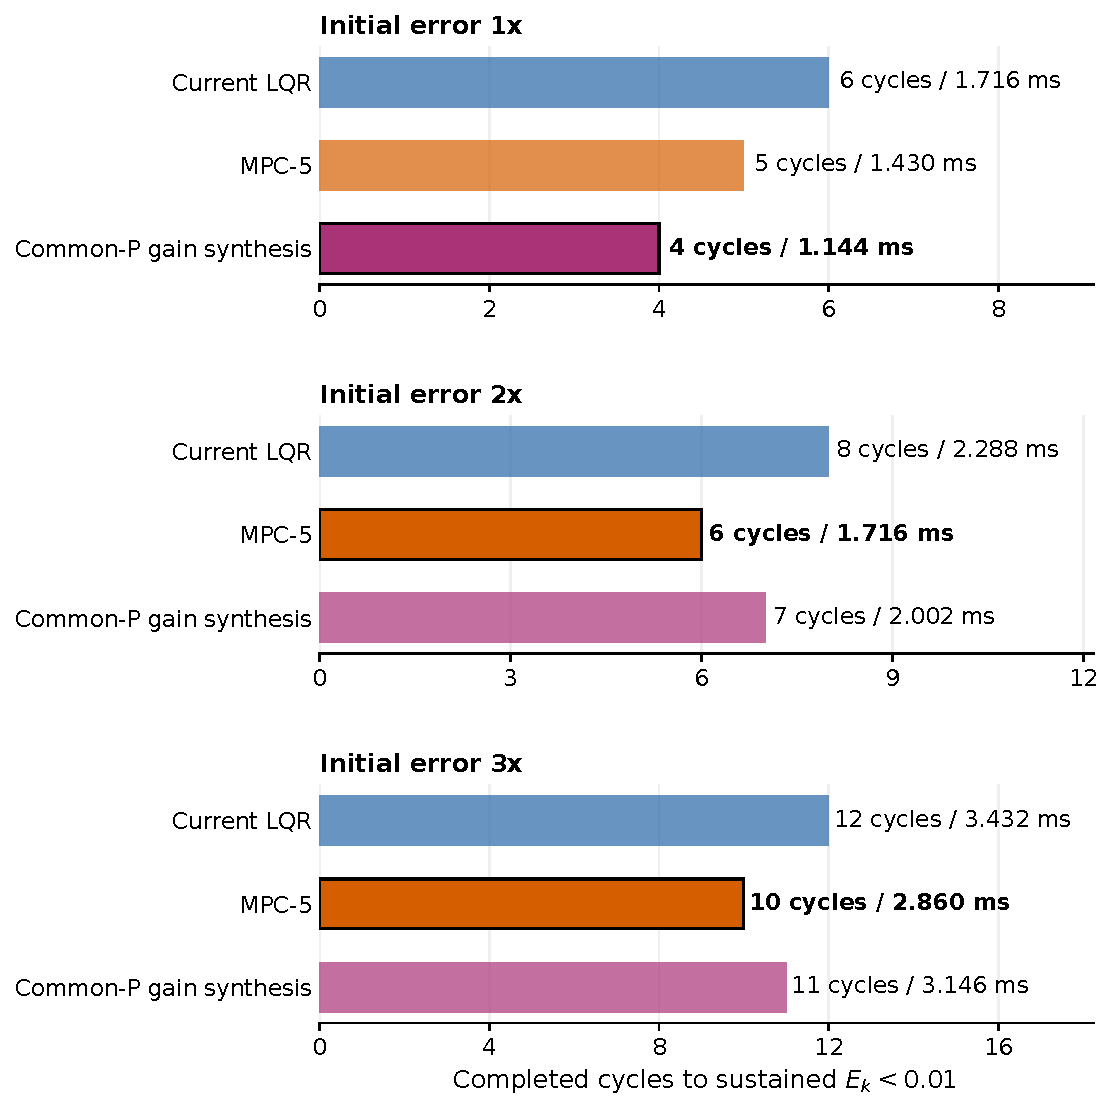
\includegraphics[width=\linewidth,height=.73\textheight,keepaspectratio]{figures/convergence_speed.pdf}
\end{center}
{\small\panelnote{\textbf{Fastest observed:} 1x: Common-P gain synthesis, 4 cycles / 1.144 ms; 2x: MPC-5, 6 cycles / 1.716 ms; 3x: MPC-5, 10 cycles / 2.860 ms.}
}

\clearpage
\section*{Convergence speed: error histories}
\panelnote{First sixteen cycles, enlarged around the $0.01$ threshold.
Circles mark the actual sustained threshold-crossing samples. The common
error is $E_k=\|S^{-1}(x_k-\bar x)\|_2$, $S=\operatorname{diag}(10,20,1)$.}
\fullfigure{convergence_errors}
\comment{The fastest controller depends on the initial-error magnitude, not only its raw closed-loop poles.}

\clearpage
\section*{Accumulated applied cost}
\panelnote{First 25 cycles. The common $J_{100}$ sums squared normalized error
and $0.001$ times squared applied offsets normalized by $10\,\mu\mathrm{s}$.
It excludes MPC's terminal penalty.}
\begin{center}
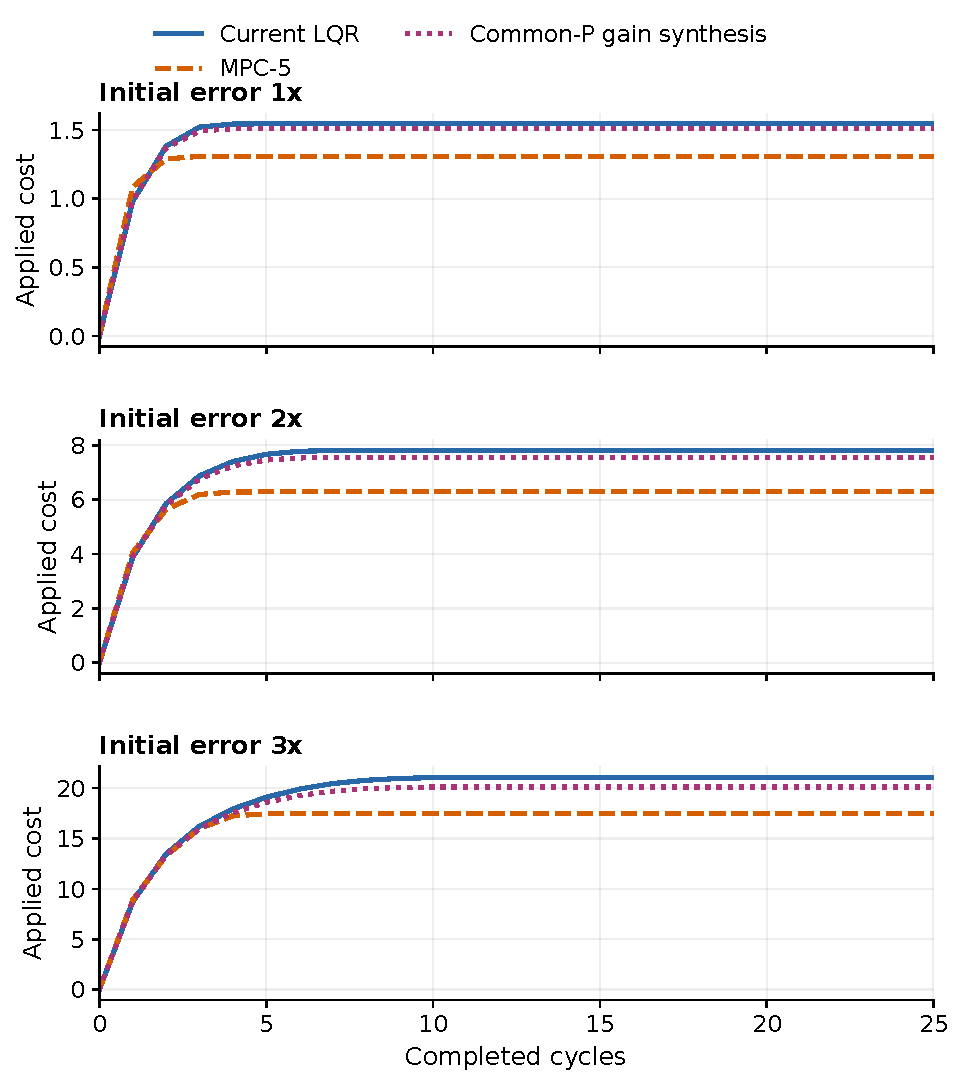
\includegraphics[width=\linewidth,height=.72\textheight,keepaspectratio]{figures/cost.pdf}
\end{center}
\begin{center}
\begin{tabular}{lrrr}
\toprule
Method & $J_{100}$, 1x & $J_{100}$, 2x & $J_{100}$, 3x \\
\midrule
Current LQR & 1.54565 & 7.80712 & 21.0741 \\
MPC-5 & 1.3099 & 6.28924 & 17.5213 \\
Common-P gain synthesis & 1.50961 & 7.54651 & 20.1221 \\
\bottomrule
\end{tabular}

\end{center}
\comment{MPC-5 has the lowest cost in all three cases. Fastest threshold crossing and lowest cost are different criteria.}

\trajectorycase{1}
\trajectorycase{2}
\trajectorycase{3}

\clearpage
\section*{How much of the static feedback is applied?}
\panelnote{The conditioning factor is shown separately for each initial-error
case. The two static gains use the same conditioner; MPC has no factor.}
\fullfigure{conditioning}
\comment{A smaller factor means more of the raw request is removed, not necessarily a slower applied response.}

\clearpage
\section*{Applied minimum dwell}
\panelnote{Each panel takes the minimum across all nine applied mode intervals.
The shaded range is forbidden. All nine compared runs respect the
$3\,\mu\mathrm{s}$ bound within numerical tolerance.}
\fullfigure{dwells}

\clearpage
\section*{Controller computation and takeaways}
\panelnote{Matched MATLAB \KawaMatlabRelease{} state-to-schedule timings:
\KawaTimingStates{} common states, \KawaTimingWarmups{} warmups and
\KawaTimingCalls{} interleaved measurements per method.}
\fullfigure{computation}
\comment{The p95 is not a worst-case bound. Desktop timing does not establish embedded deadlines.}

\subsection*{Conclusions}
\comment{Common-P gain synthesis is fastest at 1x; MPC-5 is fastest at 2x and 3x and retains the lowest cost.}
\comment{Common-P gain synthesis jointly designs the feedback gain and Lyapunov matrix through classical decay-rate LMIs, following Kawakami's suggestion. Its feasible gain is nonunique and merits more initial-error tests.}
\comment{Common-$P$ covers conditioned linearized dynamics, not global nonlinear stability or state safety.}
\panelnote{Methods and commands: \texttt{studies/kawa-synthesis/README.md}.}
\end{document}
